\documentclass[14pt]{report}
\usepackage{geometry}                % See geometry.pdf to learn the layout options. There are lots.
\geometry{letterpaper}                   % ... or a4paper or a5paper or ... 
%\geometry{landscape}                % Activate for for rotated page geometry
%\usepackage[parfill]{parskip}    % Activate to begin paragraphs with an empty line rather than an indent
\usepackage{graphicx}
\usepackage{amssymb}
\usepackage{epstopdf}
\DeclareGraphicsRule{.tif}{png}{.png}{`convert #1 `dirname #1`/`basename #1 .tif`.png}

\begin{document}
\section{Bayesian regression}
The models considered in this last section are  linear regression models. The main property of such models is that the prediction $y(x;w)$ is a linear function of weights 
\[ y(x,w) = \sum_{j=1}^{j=N} w_j\phi_j(x)    + w_0\] where $\phi_j(x)$ are basis functions

The above expression can be written in matrix form by introducing a dummy basis function  $\phi_0(x)=1$ to account the parameter $w_0$ :
\[ y(x,w) = \sum_{j=0}^{j=N} w_j\phi_j(x) =\textbf{w}^{T}\Phi \]
where $\Phi = (\phi_0,\phi_1...\phi_M)$ and $\textbf{w} =(w_0,w_1....w_M)$(M denotes the number of basis functions used)
\subsection{Part A}
\begin{figure}[h!]
  \caption{The variance of the posterior at k=1 against N }
  \centering
    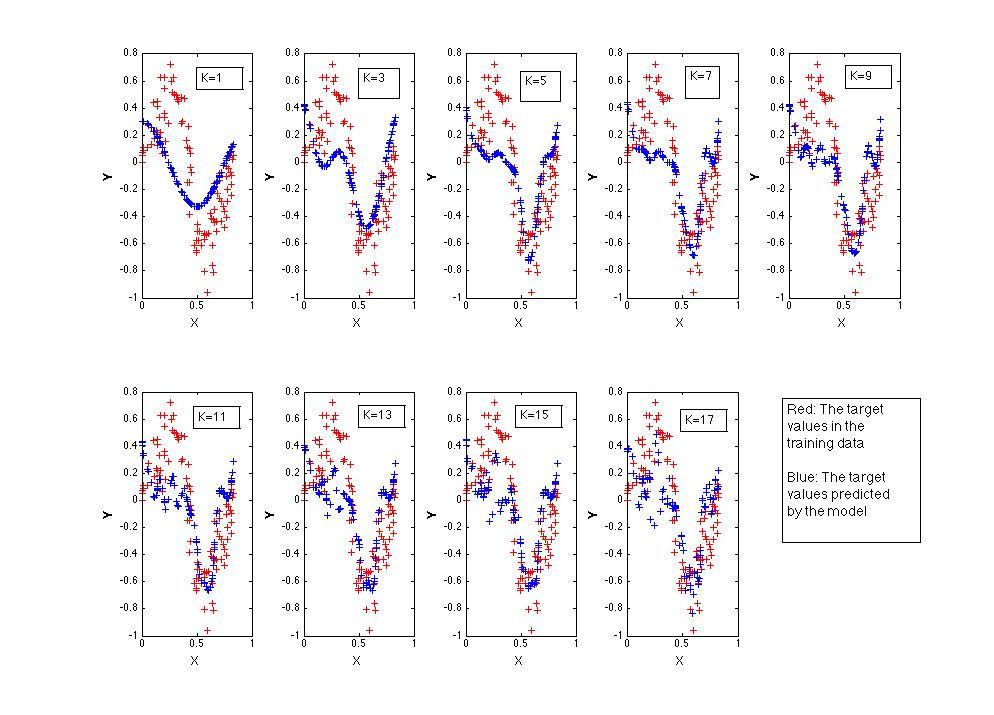
\includegraphics[width=1\textwidth]{4A.jpg}
\end{figure}
The object of Part A is to compare the performance of the prediction $y(x;w)$ on the training data given different linear models. Each model $M_i$ is distinguished from the other only in terms of the number of basis functions it employ i.e M. (All model employ fourier basis functions).



\begin{figure}[h!]
  \caption{The variance of the posterior at k=1 against N }
  \centering
    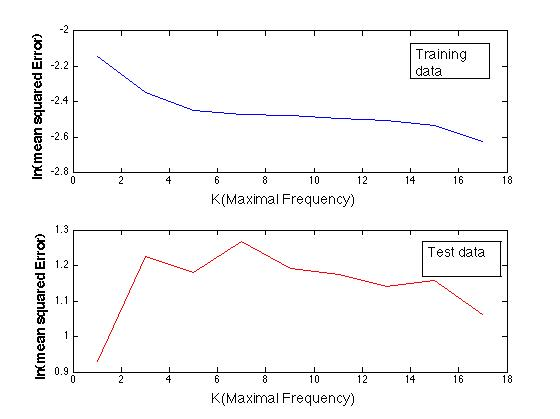
\includegraphics[width=1\textwidth]{4b.jpg}
\end{figure}
subsection{Part C}
\begin{figure}[h!]
  \caption{The variance of the posterior at k=1 against N }
  \centering
    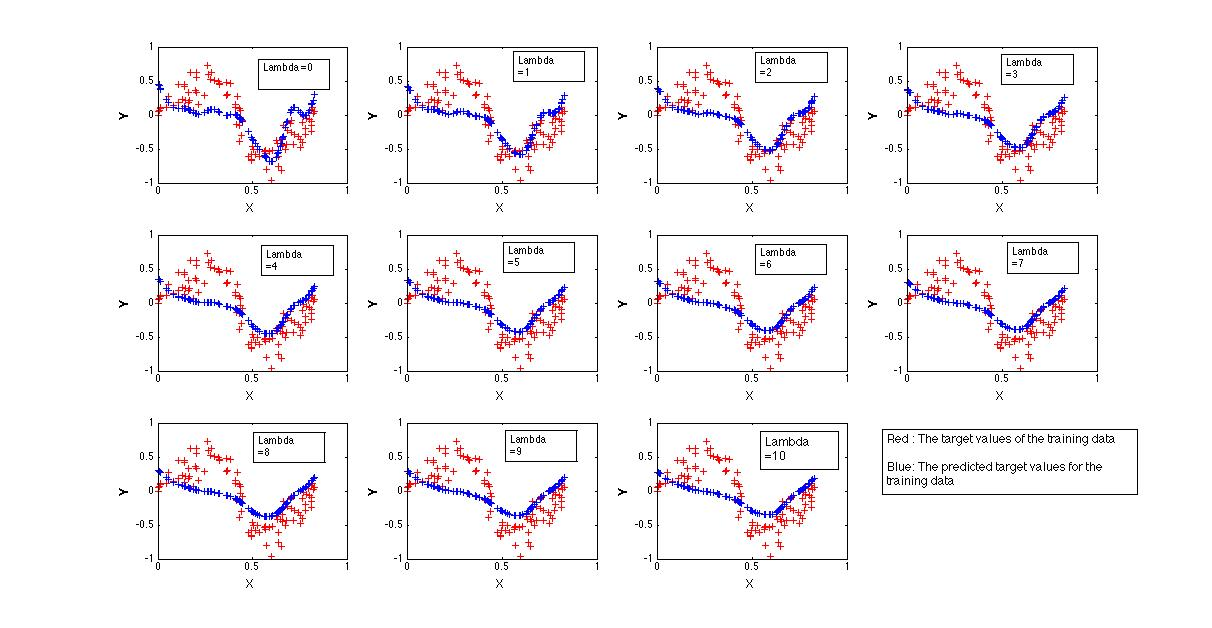
\includegraphics[width=1\textwidth]{4C.jpg}
\end{figure}
%\section{}
%\subsection{}



\end{document}  